\subsection{Overview}
\label{sec:methods-overview}

The goal of this thesis is to analyse social trends on Twitter and determine how trends spread among Croatian Twitter users over a period of time. The main challenge in conducting a data analysis is obtaining a credible dataset that allows for insightful analysis. To overcome this challenge, a \gls{data-platform} \cite{moses_gavish_2022} was created to collect, clean, transform, and apply data using a \gls{data-pipeline} developed in \gls{python} \footnote{Thesis code repository: \href{https://github.com/andhrelja/twitter\_scraper}{https://github.com/andhrelja/twitter\_scraper}}.

The following subsections describe the implementation process of the \gls{data-platform}. Work examples for the phases of the \acrfull{sdlc} are defined and described. The advantages and disadvantages of the software process models and how these methods are used to identify the created platform are shown. In addition, the ingestion, transformation and analysis processes are described in detail. This section concludes with a description of the CI/CD infrastructure.


\subsection{System Development Life Cycle}
\label{sec:methods-sdlc}
Every software development process has a starting point, but saying that it has an end point can be ambiguous. Once the software is deployed in a production environment and all \glspl{feature} have been developed, it can be assumed that the development phase is complete and the end point has been reached. At this point, software maintenance, often referred to as software support, can begin and additional system \glspl{enhancement} can be made. Maintenance usually focuses on \gls{bug} fixes or new \glspl{enhancement}, but sometimes end users may request \glspl{feature} that require additional development, which restarts the development process 

Given the cyclical nature of software processes, numerous software process models \cite{pavlic2009is} have been developed by various authors throughout history. The most famous model, the waterfall model, was introduced in the 1970s, but did not address the cyclic nature of software processes and was therefore an inefficient mechanism for software development. Over time, other models were developed to improve the rigidity of the waterfall model, leaving a variety of options to choose from to select the most appropriate software process model and create a flexible \acrlong{sdlc}. 

A software process model is used to identify the system to be built. It defines the activities for designing, implementing, testing, and monitoring software systems. Some software process models include the classic Waterfall Model, Incremental and Iterative Models and their combination, the \acrfull{rad} Model, various Prototyping Models, the Spiral model, the \acrfull{rup} Model, the V-model (verification and validation model) as an extended implementation of the Waterfall Model, and others \cite{pi2019}. The waterfall model is a precursor to other software process models, but it poses risks to the project outcome due to its linear (sequential) life cycle model.

All the models listed have similarities between the phases they define (analysis, design, development, test, and maintenance). Most models are based on an iterative life cycle model that allows for flexible requirements updates, and they are often user-driven in an \gls{agile} manner. The \gls{data-platform} created as part of this thesis is a small project guided by an implementation of iterative rapid prototyping through Analysis, Design, and Development \& Testing cycles.


\begin{center}
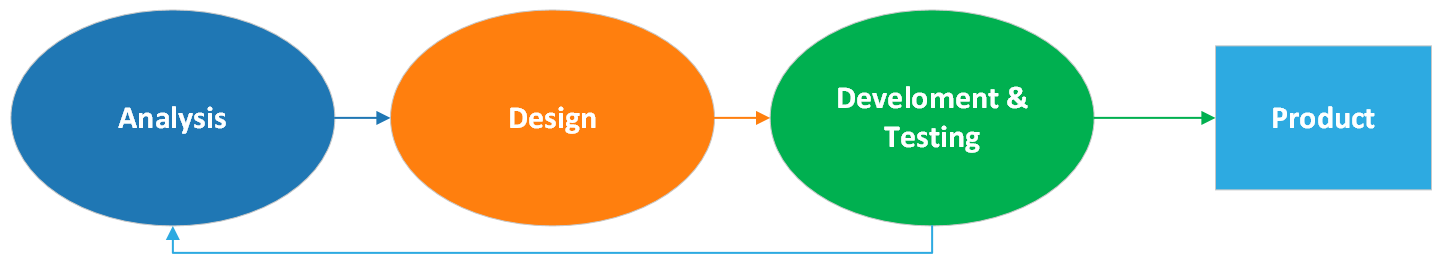
\includegraphics[width=14cm,keepaspectratio]{images/twitter-data-platform-sdlc.png}
\label{figure:twitter-data-platform-sdlc}
\captionof{figure}{Twitter \Gls{data-platform} \acrshort{sdlc}}
\end{center}

During Development \& Prototype, there was frequent switching between the analysis phase and the development and testing phase. This model has proven to be a fast development and release process, especially for features that required additional testing 

After the Testing phase demonstrates that the developed system meets the requirements of the Development \& Prototype phase, the Maintenance phase is initiated. This transition requires that data output not be compromised by developers, analysts, or others interacting with the \gls{data-platform}, so a production environment is introduced. This means that development and testing must occur as infrequently as possible and with as few changes as possible to avoid \gls{data-integrity} issues. To improve the security of the system, native GitHub functions such as \gls{branch-protection-rules} can be used.

The following subsections describe the rapid prototyping phases in the platform life cycle.

\vspace{1.2cm}
\subsubsection{Analysis}
\label{subsec:sdlc-analysis}
% \setlength\parindent{0pt}

The \textbf{goal} of this thesis is to create a dataset that provides valuable knowledge about the information being shared on Twitter and to enable analyzing social trends on Twitter through time.

Analysis phase identifies the \textbf{\gls{data-service-provider}}, \textbf{data source} endpoints, their limitations and restrictions, and finally - \textbf{data requirements}.

\paragraph{\Gls{data-service-provider}} Twitter\footnote{https://twitter.com} is the \gls{data-service-provider} for this \gls{data-platform}. The provided \acrshort{rest} service imposes various limitations and restrictions, some of them being \underline{Tweet limits} - \textit{up to 500k Tweets} are served per month and \underline{User limits} - \textit{inability to lookup Users} in a given range (location, age...). The identified limitations and restrictions need to be accounted for at the earliest stages of the Analysis phase. Failing to do so may result with disastrous effects on the product at a stage when it is too late to iterate over Analysis again. This \gls{data-platform} accounts for \underline{Tweet limits} with an option of creating multiple accounts if the \textit{500k Tweets per month} limit is surpassed and re-running the full load process (\ref{sec:methods-data-ingestion}). \underline{User limits} are accounted for by creating a baseline list of User IDs and \textit{}{expanding} it with each \gls{data-pipeline} run \textit{}{using the user's followers and friends IDs} \cite{mipro2022c19prediction}.

\paragraph{Data source} Data source endpoints are used to collect information about Twitter defined User objects and Tweet objects. Endpoints impose technical limitations, with most common limitations including a limited number of \acrshort{api} requests that an external system can make to the data source's \acrshort{rest} server. These limitations are documented in table \ref{tables:source-endpoints-limitations}.

\begin{table}[ht]
	\centering
	\begin{tabular}{ | p{4.2cm} | p{5.7cm} | p{2.6cm} | }
		\hline \textbf{Name}  & \textbf{Description}   & \textbf{Limitations} \\
		\hline
		\hline \href{https://developer.twitter.com/en/docs/twitter-api/v1/accounts-and-users/follow-search-get-users/api-reference/get-users-lookup}{users/lookup}\footnote{https://developer.twitter.com/en/docs/twitter-api/v1/accounts-and-users/follow-search-get-users/api-reference/get-users-lookup} & serves \glspl{user-object} & 900 requests / 15 minutes \\
		\hline \href{https://developer.twitter.com/en/docs/twitter-api/v1/tweets/timelines/api-reference/get-statuses-user_timeline}{statuses/user\_timeline}\footnote{https://developer.twitter.com/en/docs/twitter-api/v1/tweets/timelines/api-reference/get-statuses-user\_timeline} & serves \glspl{tweet-object} associated with a user & 900 requests / 15 minutes \\
		\hline \href{https://developer.twitter.com/en/docs/twitter-api/v1/accounts-and-users/follow-search-get-users/api-reference/get-followers-ids}{followers/ids}\footnote{https://developer.twitter.com/en/docs/twitter-api/v1/accounts-and-users/follow-search-get-users/api-reference/get-followers-ids} & serves user's follower IDs  & 15 requests / 15 minutes \\
		\hline \href{https://developer.twitter.com/en/docs/twitter-api/v1/accounts-and-users/follow-search-get-users/api-reference/get-friends-ids}{friends/ids}\footnote{https://developer.twitter.com/en/docs/twitter-api/v1/accounts-and-users/follow-search-get-users/api-reference/get-friends-ids} & serves user's friends IDs & 15 requests / 15 minutes \\
		\hline

	\end{tabular}
    \caption{Source data Endpoints Descriptions \& Limitations}
\end{table}
\label{tables:source-endpoints-limitations}

\paragraph{Data requirements} Data requirements identify the information that needs to be obtained from the data source. The \gls{data-service-provider} must be capable of satisfying the given data requirements by providing curated sets of information. The resulting \gls{data-platform} must be designed to support the given data requirements. The following bullet list provides the requirements summary:

\begin{itemize}
    \item \textbf{Users quantity}: Croatian users only
    \item \textbf{Tweets quantity}: from \texttt{2022-11-01} onward
    \item \textbf{Data re-usability}: never delete ingested data
    \item \textbf{Object details}: identify attributes that can be used to analyse social trends
\end{itemize}

Collected (\textit{ingested} afterwards) data needs to provide as much information about \textit{data source} objects as possible. This is accomplished by storing all available source object attributes and only eliminating irrelevant attributes in the \nameref{sec:methods-data-transformation} process. The ingested data is never deleted, moved or modified (in place).

The following paragraphs describes some valuable \textit{data source} object attributes and other inputs used to apply User and Tweets quantitative restrictions.

\paragraph{Location Inputs} A User object is identified as a Croatian user if their \texttt{location} attribute \textbf{contains} at least one Croatian location from \ref{methods:sdlc-inputs-locations}. As an example, if a User object's \texttt{location} attribute is set to \texttt{"Zaprešić"}, he will be identified as a Croatian user because (\texttt{"Zaprešić"} is a subset of \texttt{"Zaprešić,Croatia"} \textbf{or} \texttt{"Zaprešić,Croatia"} is a subset of \texttt{"Zaprešić"}). 


\begin{code}
\captionof{listing}{Croatian Locations Input} 
\label{methods:sdlc-inputs-locations}
\begin{minted}[frame=single,
               framesep=3mm,
               tabsize=2]{js}
[
    "Hrvatska",
    "Croatia",
    "Žminj",
    "Zaprešić,Croatia",
    "Virovitica",
    "republic of dalmatia baby!",
    "velika gorica, croatia",
    "RIJEKA"
]
\end{minted}
\end{code}

The \nameref{methods:sdlc-inputs-locations} was derived manually by inspecting the \nameref{subsubsec:sdlc-analysis-data-source:ingest-user}'s \texttt{location} attribute values and capturing them in a separate \acrshort{json} file. The values were only inspected once and the input locations were not revised since. 

Additional transformations were performed on \nameref{methods:sdlc-inputs-locations} to ensure Users are correctly identified as Croatian users. Some transformations include converting the \texttt{location} strings to lowercase, punctuation and diacritics removal and white-space and Unicode character removal. 

These operations were simple to execute on this input file, but they were time-expensive when applied to the User models and they did not yield results that would justify their use. After performing this due diligence, the additional transformation functionality was discarded and it is no longer in use.



\paragraph{Ingested Users} The User object contains a large number of attributes. Only a subset of attributes are presented and described, but all of them are ingested. Details about all attributes can be found at the Twitter's \href{https://developer.twitter.com/en/docs/twitter-api/v1/data-dictionary/object-model/user}{Tweet object}\footnote{https://developer.twitter.com/en/docs/twitter-api/v1/data-dictionary/object-model/user} page.

\clearpage
\begin{code}
\captionof{listing}{Ingest User}
\label{subsubsec:sdlc-analysis-data-source:ingest-user}
\begin{minted}[frame=single,
               framesep=3mm,
               tabsize=2]{js}
{
    "name": "HNS",
    "screen_name": "HNS_CFF",
    "location": "Hrvatska | Croatia",
    "description": "Službeni Twitter profil Hrvatskog"
                   "nogometnog saveza Croatian Football"
                   "Federation official Twitter feed."
                   "#HNS #Obitelj #Family",
    "protected": false,
    "followers_count": 262456,
    "friends_count": 116,
    "statuses_count": 19515
}
\end{minted}
\end{code}

\begin{itemize}
    \item \texttt{name}: The name of the user, as they have defined it. Not necessarily a person's name
    \item \texttt{screen\_name}: The screen name, handle, or alias that this user identifies themselves with. \texttt{screen\_names} are unique but subject to change
    \item \texttt{location}: \textit{Nullable}. The user-defined location for this account's profile
    \item \texttt{description}: \textit{Nullable}. The user-defined UTF-8 string describing their account
    \item \texttt{protected}: When true, indicates that this user has chosen to protect their Tweets (\href{https://help.twitter.com/en/managing-your-account/about-twitter-verified-accounts}{Verified Accounts}\footnote{https://help.twitter.com/en/managing-your-account/about-twitter-verified-accounts})
    \item \texttt{followers\_count}: The number of followers this account currently has
    \item \texttt{friends\_count}: Number of accounts that the user follows
    \item \texttt{statuses\_count}: The number of users this account is following (also known as their \texttt{"followings"})
\end{itemize}


\clearpage
\paragraph{Ingested Tweets} Twitter uses the term \textit{status} when referring to a Tweet. The Tweet object contains a large number of attributes. Only a subset of attributes are presented and described, but the entire set is ingested. Details about all attributes can be found at the Twitter's \href{https://developer.twitter.com/en/docs/twitter-api/v1/data-dictionary/object-model/tweet}{Tweet object}\footnote{https://developer.twitter.com/en/docs/twitter-api/v1/data-dictionary/object-model/tweet} page.

\begin{code}
\captionof{listing}{Ingest Tweet}
\label{subsubsec:sdlc-analysis-data-source:ingest-tweet}
\begin{minted}[frame=single,
               framesep=3mm,
               tabsize=2]{js}
{
    "created_at": "Tue Nov 22 10:00:18 +0000 2022",
    "full_text": "VATRENI IS LISTED"
                 "\n\nThis is truly a historic moment"
                 "because #VATRENI is so much more "
                 "than just a token. Become a part"
                 "of the greatest fan story and enjoy"
                 "all kinds of benefits.\n\n#VATRENI"
                 "token is now live at @gate_io \n\n",
    "entities": {
        "hashtags": [
            {"text": "VATRENI"},
            {"text": "VATRENI"}
        ],
        "user_mentions": [
            {"id": 912539722, "screen_name": "gate_io"}
        ]
    },
    "user": { ingested_user },
    "retweet_status": { ingested_tweet },
    "in_reply_to_status_id": null,
    "in_reply_to_user_id": null,
    "quoted_status": { ingested_tweet },
    "favorite_count": 41,
    "possibly_sensitive": false,
    "lang": "en"
}
\end{minted}
\end{code}

\begin{itemize}
    \item \texttt{created\_at}: UTC time when this Tweet was created
    \item \texttt{full\_text}: The actual UTF-8 text of the status update
    \item \texttt{entities}: Entities which have been parsed out of the text of the Tweet. Additionally see \href{https://developer.twitter.com/overview/api/entities-in-twitter-objects}{Entities in Twitter objects}\footnote{https://developer.twitter.com/overview/api/entities-in-twitter-objects}
        \begin{itemize}
        \item \texttt{hashtags}: Names of the hashtags used in this Tweet, minus the leading \texttt{"\#"} character
        \item \texttt{user\_mentions}: IDs of the mentioned users, as an integer
        \end{itemize}
    \item \texttt{user}: Ingested User (\nameref{subsubsec:sdlc-analysis-data-source:ingest-user})
    \item \texttt{retweet\_status}: Retweets can be distinguished from typical Tweets by the existence of a retweeted\_status attribute. This attribute contains a representation of the original Tweet that was retweeted (\nameref{subsubsec:sdlc-analysis-data-source:ingest-tweet})
    \item \texttt{in\_reply\_to\_status\_id}: \textit{Nullable}. If the represented Tweet is a reply, this field will contain the integer representation of the original Tweet's ID
    \item \texttt{in\_reply\_to\_user\_id}: \textit{Nullable}. If the represented Tweet is a reply, this field will contain the integer representation of the original Tweet's author ID
    \item \texttt{is\_quote\_status}: Indicates whether this is a Quoted Tweet
    \item \texttt{quoted\_status}: This attribute contains a representation of the original Tweet that was quoted (\nameref{subsubsec:sdlc-analysis-data-source:ingest-tweet}). Quote tweets are Retweets that contain some original content (\texttt{full\_text}, \texttt{hashtagas}, \texttt{user\_mentions})  
    \item \texttt{favorite\_count}: \textit{Nullable}. Indicates approximately how many times this Tweet has been liked by Twitter users
    \item \texttt{possibly\_sensitive}: \textit{Nullable}. This field indicates content may be recognized as sensitive. This may also be judged and labeled by an internal Twitter support agent
    \item \texttt{lang}: \textit{Nullable}. When present, indicates a \href{http://tools.ietf.org/html/bcp47}{BCP 47}\footnote{http://tools.ietf.org/html/bcp47} language identifier corresponding to the machine-detected language of the Tweet text, or und if no language could be detected
\end{itemize}



\clearpage
\subsubsection{Design}
\label{subsec:sdlc-design}

Design phase focuses on shaping the mechanisms by which data is ingested and transformed to create a dataset that can be easily used for data analysis 

The resulting \gls{data-platform} must support storage of the full raw data as-is, without any changes being made in the ingestion process (\ref{sec:methods-data-ingestion}). The transformation process uses the full data set to apply filters and changes to the raw data. This process performs read operations on the ingested data, transforms \gls{in-memory} data, and stores the resulting dataset in a new location that is independent of the ingestion location. Before the resulting dataset is stored, it is filtered to contain only Croatian users, and the baseline list of User IDs is overwritten with the available Croatian user IDs. Figure \ref{figure:twitter-data-platform-design} shows an overview of the implemented \gls{data-platform} architecture.

\begin{center}
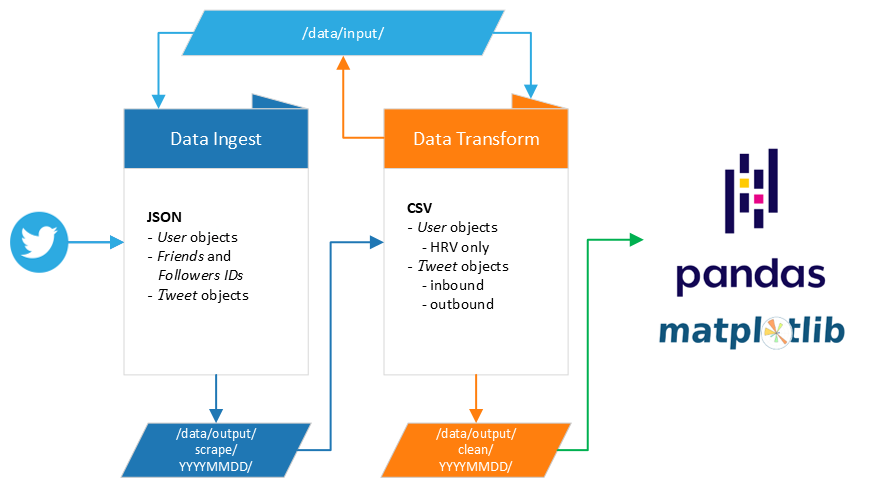
\includegraphics[width=14cm,keepaspectratio]{images/twitter-data-platform.png}
\label{figure:twitter-data-platform-design}
\captionof{figure}{Twitter \Gls{data-platform} Architecture}
\end{center}

Both ingestion and transformation output locations (in particular, the directories reflecting the ingestion date) are created at runtime. This mechanism allows the ingested and transformed data to be examined per ingestion date, and ensures that only the most recently ingested data is transformed, rather than the entire data for each \gls{data-pipeline} run. The resulting dataset is a union of all files in the date directories in the output file system of the data conversion and is analysed (\ref{sec:methods-data-analysis}) using the \gls{pandas} and \gls{matplotlib} tools.

\paragraph{Data target filesystem} A filesystem is used to store data throughout the \gls{data-pipeline}. The data is stored on an on-premise Linux server provided by the University of Rijeka. The filesystem includes two main directories: \texttt{input} and \texttt{output}. The \texttt{output} directory is then divided into the \texttt{scrape} ( ingested data) and \texttt{clean} (transformed data) directories, partitioned by date.
\vspace{0.6cm}
\begin{figure}[hb]
\dirtree{%
.0 data.
    .1 input.
        .2 locations.
            .3 hr.json.
    .1 output.
        .2 scrape.
            .3 tweets.
                .4 2022-11-01.
            .3 users.
                .4 ids.
                    .5 2022-11-01.
                .4 objs.
                    .5 2022-11-01.
        .2 clean.
            .3 tweets.
                .4 2022-11-01.
            .3 users.
                .4 2022-11-01.
}
\caption{Data target file system structure}
\end{figure}
\label{tabels:target_fs}


\vspace{1.2cm}
\subsubsection{Development \& Testing}
\label{subsec:sdlc-development}

Development (Prototyping) \& Testing phase is focused on developing the mechanisms used to ingest, and transform data defined in the \nameref{subsec:sdlc-design} phase. This phase ensures that ingestion and transformation are independent (\gls{loosely-coupled}) processes, that enable historical and incremental data ingestion, notification mechanism and CI/CD mechanisms (\ref{sec:methods-cicd}).


\vspace{1.2cm}
\subsubsection{Maintenance}
\label{subsec:sdlc-maintenance}

Maintenance phase focuses on supporting the end-users in their \gls{data-platform} usage. Once Development \& Testing is completed and the system is deployed to \textit{production}, it is maintained to ensure that any unexpected \glspl{bug} are promptly fixed and supported to accommodate new \glspl{enhancement}. This phase may also support \gls{feature} development requests, but if a development effort exceeds the scope of the defined Design, a new iteration is initiated across \acrshort{sdlc} phases.


\clearpage
\subsection{Data Ingestion}
\label{sec:methods-data-ingestion}
Data ingestion is the process of obtaining data from a \textit{data source} to its home system as efficiently and correctly as possible~\cite{meehan2017data}. Home system in the context of this thesis is a \gls{file-system} used as a part of the developed \gls{data-platform}. A \textit{data source} is a place where information is obtained - the source can be a database, a \gls{flat-file}, an XML file, or any other format an \gls{operating-system} can read.

The \textit{data source} used by this thesis is Twitter, offering a \gls{rest-api} service to serve their data. High volume of data generated on Twitter makes it difficult for the \acrshort{rest} service to enable high \gls{data-availability}, so Twitter limits the amount of data that can be collected per user (e.g. only the \textbf{latest 3,200} user's tweets can be obtained). To support historic data storage - the collected data is continuously collected and never deleted.

Data ingestion architecture depends on the \textit{data source} system type and the \nameref{sec:methods-data-analysis} requirements. Four common architecture patterns are described in the following paragraphs.

\hfill

\paragraph{Real-Time Ingestion} Real-Time Ingestion is usually used for \gls{real-time-data}. It applies simultaneous intermittent processing to data in small sizes (order of Kilobytes). This is an \gls{event-based} ingestion system.

\paragraph{Streaming Ingestion} Streaming Ingestion is usually used for \gls{streaming-data}. It applies simultaneous continuous processing of data in small sizes (order of Kilobytes). This is an \gls{event-based} ingestion system.
 
\paragraph{Batch Ingestion} Batch Ingestion is usually used for \gls{big-data}. It applies non-simultaneous processing of data in large sizes (batches, order of Megabytes). This is a \gls{schedule-based} ingestion system.

\paragraph{Lambda Architecture} \gls{lambda-architecture} is usually used for a combination of \gls{streaming-data} and \gls{big-data}. It applies simultaneous and non-simultaneous processing of data in all sizes. This can be \gls{event-based} and \gls{schedule-based} ingestion system.

\hfill

Twitter \textit{data source} provides both \gls{real-time-data} and \gls{big-data}. Real-time ingestion is not required by the \nameref{sec:methods-data-analysis} for this \gls{data-platform} because \glspl{data-analyst} conduct their analysis on weekly or monthly bases. Given the requirements, the \textbf{batch ingestion} architecture pattern is selected to guide the \textit{design} for this \gls{data-platform}, with the ingestion schedule set for every \textbf{Monday at 12AM UTC}.

After the architecture pattern is curated, the methods for moving the data need to be defined. It is important to note that all architecture patterns require data movement methods, but each pattern only supports a subset of data movement methods. Two of the most commonly used data movement methods for batch ingestion are described in the following paragraphs.

\hfill

\paragraph{Full Load} Full loads are also known as \textit{Historic} loads. They takes place the first time a data source is loaded into the home system.

\paragraph{Incremental Load} Incremental loads are also known as \textit{Delta} loads. They take place on each subsequent time a data source is loaded into the home system. Delta loads are usually tracked by a date and time value (last received record date and time, last historic or incremental load date and time and similar) for the next incremental load to correctly identify the starting point of the data being collected.

\hfill

This \gls{data-platform} supports full and incremental data movement methods. Because of the Twitter \acrshort{rest} limitation where only the latest 3,200 user's tweets can be obtained, it is essential that the collected data is stored and never deleted. If the collected data gets deleted, it is unrecoverable because Twitter will never serve the user's 3,201\textsuperscript{st} tweet using the current version of their \acrshort{rest} service again.

\clearpage

By creating software support for incremental loads, support for full loads is implied. The \gls{data-pipeline} reads the following \acrshort{json} inputs to determine what is the starting point of the data being moved:

\begin{itemize}
    \item \texttt{baseline-user-ids}: array of user IDs, manually created to collect tweets from
    \item \texttt{processed-user-objs}: array of user IDs, processed in a previous ingestion
    \item \texttt{missing-user-objs}: array of user IDs, non-existing profiles for a given user ID
    \item \texttt{max-tweet-ids}: object, last received tweet record for a user represented by a key-value pair (\texttt{\{user ID: last tweet ID\}})
    \vspace{0.6cm}
\end{itemize}


First time the data is loaded into the home system, the full load takes place collecting the manually created \texttt{baseline-user-ids}. At this point, the remaining inputs still do not exist. After the first user ID is processed, the respective user object is created, adding the processed user ID to \texttt{processed-user-objs}. Once all the users are processed, they are filtered to Croatian users only (using the \nameref{methods:sdlc-inputs-locations} \acrshort{json} input) within the \nameref{sec:methods-data-transformation} process, the \texttt{baseline-user-ids} gets updated with the Croatian user IDs and the tweet ingestion starts. Since there isn't a \texttt{max-tweet-ids} to determine the last received user's tweet, all the latest \(3,200\) user's tweets (from today) until \texttt{2022-11-01 00:00 UTC} are obtained and the \texttt{max-tweet-ids} file is created.

All the next loads are incremental ones, reading inputs created by the full load. Incremental loads only collect the \texttt{baseline-user-ids} that do not exist in \texttt{processed-user-objs} and \texttt{missing-user-objs}.


\clearpage
\subsection{Data Transformation}
\label{sec:methods-data-transformation}
Data transformation is the process of converting data from one format or structure into another format or structure. This is often done to make the data more useful or easier to work with for specific purposes, such as analysis or machine learning. Data transformation can involve a wide range of techniques, such as cleaning and preprocessing, normalization, aggregation, and feature extraction. The specific steps involved in a data transformation process will depend on the specific data and the desired end result.

The data transformation process applied to the collected data is designed to be re-runnable in a way that does not affect the stored raw data. This process usually consumes a large amount of time, so it only runs once. The transformed data is then reused throughout the \ref{sec:methods-data-analysis} process. To support the given data requirements, the transformation process filters all collected Users to Croatian users only (\nameref{methods:sdlc-inputs-locations}) and applies other filters (\texttt{statuses\_count > 10}, \texttt{followers\_count > 10}, \texttt{friends\_count > 10} and similar), to ensure the collected Users represent a legitimate sample.

The resulting transformed data is used to create \glspl{data-view} to be used by the \Glspl{data-analyst}.

\begin{code}
\captionof{listing}{Transform User}
\label{subsubsec:sdlc-analysis-data-transformations:transform-user}
\begin{minted}[frame=single,
               framesep=3mm,
               tabsize=2]{js}
{
    "name": "HNS",
    "screen_name": "HNS_CFF",
    "location": "Croatia",
    "is_croatian": true,
    "description": "Službeni Twitter profil Hrvatskog"
                   "nogometnog saveza Croatian Football"
                   "Federation official Twitter feed."
                   "#HNS #Obitelj #Family",
    "followers_count": 253625,
    "friends_count": 117,
    "statuses_count": 19209,
    "created_at": "2022-08-30T05:56:36+00:00"
}
\end{minted}
\end{code}

The User object contains a small number of transformations compared to the Tweet object. The following attributes and transformations are applied to the User object:

\begin{itemize}
    \item \texttt{location}: \underline{extract} city name text value if it is included in the original value, otherwise set to \texttt{Hrvatska}
    \item \texttt{is\_croatian}: \underline{create} boolean value to indicate whether or not the user is from Croatia 
    \item \texttt{description}: User provided profile description
    \item \texttt{followers\_count}: number of users following this User
    \item \texttt{friends\_count}: number of users this User follows
    \item \texttt{statuses\_count}: total number of published Tweets since \texttt{created\_at}
    \item \texttt{created\_at}: \underline{evaluate} string to date-time object; represents profile creation date and time
\end{itemize}

\clearpage
\begin{code}
\captionof{listing}{Transform Tweet}
\label{subsubsec:sdlc-analysis-data-transformations:transform-tweet}
\begin{minted}[frame=single,
               framesep=3mm,
               tabsize=2]{js}
{
    "created_at": "2022-11-22 10:00:18+00:00",
    "created_at_year": 2022,
    "created_at_month": 11,
    "created_at_week": 47,
    "created_at_day": 22,
    "full_text": "VATRENI IS LISTED"
                 "\n\nThis is truly a historic moment"
                 "because #VATRENI is so much more "
                 "than just a token. Become a part"
                 "of the greatest fan story and enjoy"
                 "all kinds of benefits.\n\n#VATRENI"
                 "token is now live at @gate_io \n\n"
                 "Get it here: "
                 "https://t.co/sN8mWtUac6"
                 "https://t.co/XfqNfwUeCS",
    "hashtags": ["VATRENI", "VATRENI"],
    "user_mentions": ["gate_io"],
    "is_retweet": true,
    "retweet_count": 15,
    "retweet_created_at": "2022-11-22 10:29:47+00:00",
    "retweet_from_tweet_id": 1594994170858463232,
    "retweet_from_user_name": "vatreni_token",
    "retweet_timedelta_sec": 960,
    "is_reply": false,
    "reply_to_tweet_id": null,
    "reply_to_user_name": null,
    "is_quote": false,
    "favorite_count": 41,
    "possibly_sensitive": false,
    "lang": "en",
    "transform_date": "2022-11-22"
}
\end{minted}
\end{code}

The Tweet object contains a large number of transformations. The following attributes and transformations are applied to the Tweet object:

\begin{itemize}
    \item \texttt{created\_at\_year}: \underline{extract} year number from \texttt{created\_at}
    \item \texttt{created\_at\_month}: \underline{extract} month number from \texttt{created\_at}
    \item \texttt{created\_at\_week}: \underline{extract} week number from \texttt{created\_at}
    \item \texttt{created\_at\_day}: \underline{extract} day number from \texttt{created\_at}
    \item \texttt{hashtags}: \underline{extract} hashtag text from \texttt{entities.hashtags}
    \item \texttt{user\_mentions}: \underline{extract} mentioned user's screen\_name from \\ 
    \texttt{entities.user\_mentions}
    \item \texttt{is\_retweet}: \underline{create} boolean value based on existence of \\
    \texttt{retweeted\_status}
    \item \texttt{retweet\_count}: \underline{create} numeric value based on all other Tweet objects where their \texttt{retweeted\_status.id} equals this Tweet object's \texttt{id}
    \item \texttt{retweet\_created\_at}: \underline{extract} date-time object from \\
    \texttt{retweeted\_status.created\_at}
    \item \texttt{retweet\_from\_tweet\_id}: \underline{extract} numeric Tweet identifier from \\
    \texttt{retweeted\_status.id}
    \item \texttt{retweet\_from\_user\_name}: \underline{extract} text User identifier from \\
    \texttt{retweeted\_status.user.user\_id}
    \item \texttt{retweet\_timedelta\_sec}: \underline{create} \href{https://pandas.pydata.org/docs/reference/api/pandas.Timedelta.html}timedelta\footnote{https://pandas.pydata.org/docs/reference/api/pandas.Timedelta.html} value based on the difference between \texttt{retweet\_created\_at} and \texttt{created\_at}
    \item \texttt{is\_reply}: \underline{create} boolean value based on existence of \\
    \texttt{in\_reply\_to\_status\_id}
    \item \texttt{reply\_to\_tweet\_id}: \underline{rename} \texttt{in\_reply\_to\_status\_id}
    \item \texttt{reply\_to\_user\_name}: \underline{rename} \texttt{in\_reply\_to\_screen\_name}
    \item \texttt{is\_quote}: \underline{rename} \texttt{is\_quote\_status}
    \item \texttt{lang}: \underline{apply} a language detection function using \href{https://github.com/saffsd/langid.py}{langid}\footnote{https://github.com/saffsd/langid.py} if the original value was undefined
    \item \texttt{transform\_date}: \underline{create} text value based on the transformation date
\end{itemize}


\clearpage
\subsection{Data Analysis}
\label{sec:methods-data-analysis}
Data analysis is a process of inspecting, cleansing, transforming, and modeling data with the goal of discovering useful information, informing conclusions, and supporting decision-making \cite{brown2014transforming}. It is usually conducted by a \Gls{data-analyst}. Depending on the context to which the term is applied, data analysis can imply additional methods such as ingesting, transforming, modeling or other data processing methods. Within the context of this thesis, data analysis includes preprocessing transformed data, analysing it and interpreting the analysis to draw conclusions about the ways users share information and what information they share on this social network.

In statistical applications, data analysis can be divided into descriptive statistics, \acrfull{eda}, and \acrfull{cda} \cite{leech2015spss}. Descriptive statistics is the process of using and analysing quantitative descriptions or feature\footnote{The terms \textit{attribute}, \textit{field}, and \textit{column} from previous sections are synonyms to the term \textit{feature}. The main difference between the terms is that \glspl{data-analyst} tend to use the term \textit{feature} to empathize the importance of an \textit{attribute}} summaries from a collection of information \cite{mann1995introductory}. \acrshort{eda} focuses on discovering new features in the data while \acrshort{cda} focuses on confirming or rejecting existing hypotheses. Additionally, in social networks and similar applications, graph analytics is frequently used to observe the relationships between objects which are being analysed.

The analysis conducted as a part of this thesis combines descriptive statistics, \acrshort{eda} and graph analysis approaches to describe the available dataset, summarize its main characteristics and derive new \glspl{data-view} that allow for tracking social trends on Twitter through time. In the scope of this thesis, a trend is defined as a set of topics consisting of hashtags (often referred to as Tweet content).


\subsubsection{Descriptive Statistics}
\label{subsubsec:methods-data-analysis:descriptive-statistics}

Descriptive statistics applications include data statistics calculation techniques to provide a quantitative summary of the analysed data. Additional data metrics include the earliest and latest tweet date and time (\texttt{2022-11-01 00:00:12+00:00} - \texttt{2022-11-30 23:59:52+00:00}), total number of tweets (\(386,168\)), number of all Croatian Users (\(48,954\)) and the number of Users who are active within the described time range (\(6,887\)). Additional information available in Appendix\ref{part:appendix}. Table \ref{sec:data-analysis:descriptive-statistics:stat-desc}. provides a summary about the measures of the data. Some information that can be interpreted is the average number of followers a user has (\texttt{mean} of \texttt{followers\_count}: \(1,408.73\), however this average is unreliable because of a high \gls{standard-deviation} - the \texttt{90\%} column shows that the least amount of users has the most followers) and the average number of original tweets a user posted (\textit{mean} of \texttt{original\_tweets\_cnt}: \(95.34\)). It is surprising to see that only a small group of users' tweets get retweeted or quoted (\textit{mean} of \texttt{in\_retweet\_cnt}: \(2.67\), \texttt{in\_quote\_cnt}: \(1.0\)). Related works on the topic of Twitter analysis have shown that retweets are the most common way of spreading information on Twitter \cite{mestrovic2022retweetprediction}, so it can be expected that the information spread among Croatian Twitter Users is seeded from a very small number of users - those with the highest retweets count. 

\begin{table}[hb]
\caption{Statistical measures describing numeric data features in Users, post preprocessing}
\label{sec:data-analysis:descriptive-statistics:stat-desc}
\resizebox{\columnwidth}{!}{\begin{tabular}{l|r|r|r|r|r|r|r|r|r}
 & count & mean & std & min & 30\% & 60\% & 90\% & max \\
\hline
followers\_count & 6,887 & 1,408.73 & 21,214.16 & 11.0 & 68.0 & 262.0 & 1,662.8 & 1,541,746.0 \\
friends\_count & 6,887 & 568.93 & 751.9 & 11.0 & 168.0 & 410.0 & 1,334.6 & 5,002.0 \\
total\_out\_tweets\_cnt & 6,887 & 138.76 & 396.97 & 1.0 & 7.0 & 34.0 & 320.0 & 5,342.0 \\
original\_tweets\_cnt & 6,887 & 95.34 & 298.68 & 0.0 & 3.0 & 19.0 & 211.0 & 5,337.0 \\
out\_retweet\_cnt & 6,887 & 43.41 & 216.0 & 0.0 & 0.0 & 5.0 & 65.0 & 5,093.0 \\
out\_reply\_cnt & 6,887 & 59.38 & 221.26 & 0.0 & 1.0 & 7.0 & 127.0 & 5,180.0 \\
out\_quote\_cnt & 6,887 & 8.89 & 48.69 & 0.0 & 0.0 & 1.0 & 15.0 & 1,479.0 \\
out\_retweet\_timedelta\_sec & 4,598 & 809,044.12 & 6,993,425.17 & 8.5 & 26,884.7 & 62,736.0 & 948,475.5 & 315,960,857.0 \\
out\_quote\_timedelta\_sec & 2,344 & 1,717,686.97 & 10,939,711.03 & 20.33 & 20,514.07 & 66,729.8 & 1,786,563.6 & 281,322,829.8 \\
\hline
total\_in\_tweets\_cnt & 6,887 & 16.18 & 75.21 & 0.0 & 0.0 & 1.0 & 28.0 & 1,844.0 \\
in\_retweet\_cnt & 6,887 & 2.67 & 22.95 & 0.0 & 0.0 & 0.0 & 3.0 & 1,266.0 \\
in\_reply\_cnt & 6,887 & 12.69 & 62.69 & 0.0 & 0.0 & 0.0 & 19.0 & 1,499.0 \\
in\_quote\_cnt & 6,887 & 0.82 & 6.13 & 0.0 & 0.0 & 0.0 & 1.0 & 374.0 \\
in\_original\_favorite\_cnt & 6,887 & 581.45 & 6,796.17 & 0.0 & 1.0 & 22.0 & 661.0 & 458,954.0 \\
in\_retweet\_favorite\_cnt & 6,887 & 910,049.29 & 5,439,527.81 & 0.0 & 0.0 & 12,987.0 & 1,342,942.2 & 198,673,449.0 \\
in\_quote\_favorite\_cnt & 6,887 & 128,179.92 & 711,156.8 & 0.0 & 0.0 & 0.0 & 139,581.6 & 21,591,725.0 \\
in\_retweet\_timedelta\_sec & 6,887 & 1,150.15 & 14,274.44 & 0.0 & 0.0 & 0.0 & 440.07 & 793,138.2 \\
in\_quote\_timedelta\_sec & 6,887 & 235.93 & 2,114.61 & 0.0 & 0.0 & 0.0 & 49.93 & 82,308.88 \\
\hline
\end{tabular}}

\end{table}



\subsubsection{Exploratory Data Analysis}
\label{subsubsec:methods-data-analysis:eda}

\acrshort{eda} applications include \gls{data-preprocessing} and \gls{data-visualization} techniques to provide valuable data insights and allow for different types of Data Analysis. \Gls{data-preprocessing} was an integral part to the conducted analysis as it provided deeper insights into User interactions with Tweets, by aggregating tweets data. Produced aggregations expanded the original User and Tweets objects with information about the user's outbound (how many tweets they published and count of favorites the user gave out) and inbound (how many other users retweeted or quoted this user and count of favorites the user received) interactions, supporting drill-downs through date and time, hashtags and user mentions. Twitter object \ref{subsubsec:methods-data-analysis:eda:expand-user}. describes a User object after it was preprocessed. 

\clearpage
\begin{code}
\captionof{listing}{Preprocessed User object}
\label{subsubsec:methods-data-analysis:eda:expand-user}
\begin{minted}[frame=single,
               framesep=3mm,
               tabsize=2]{js}
{
  "screen_name": "HNS_CFF",
  "followers_count": 253625,
  "friends_count": 117,
  "original_tweets_cnt": 670.0,
  
  "total_out_tweets_cnt": 779.0,
  "out_retweet_cnt": 109.0,
  "out_reply_cnt": 2.0,
  "out_quote_cnt": 119.0,
  "out_retweet_timedelta_sec": 4978.899083,
  "out_quote_timedelta_sec": 18670.231707,
  
  "total_in_tweets_cnt": 1248.0,
  "in_retweet_cnt": 1266.0,
  "in_reply_cnt": 204.0,
  "in_quote_cnt": 374.0,
  "in_retweet_timedelta_sec": 5720.02172,
  "in_quote_timedelta_sec": 2261.416613,  
  
  "in_original_favorite_cnt": 209617.0,
  "in_retweets_favorite_cnt": 277942.0,
  "in_quotes_favorite_cnt": 418973.0,

  "original_hashtags":  [ "FIFAWorldCup", "Family"],
  "retweet_hashtags":   [ "MiaSanMia", "FCBayern"],
  "quote_hashtags":     [ "ForzaInter", "dinamozagreb"],
  
  "original_user_mentions": [ "lukamodric10", "DalicZlatko"],
  "retweet_user_mentions":  [ "HNS_CFF",  "lukamodric10"],
  "quote_user_mentions":    [ "lukamodric10",  "staderennais"]
}

\end{minted}
\end{code}

\clearpage
\subsubsection{Graph Analytics}
\label{subsubsec:methods-data-analysis:graph-analysis}

Graph analytics, or Graph algorithms, are analytic tools used to determine the strength and direction of relationships between objects in a graph. The focus of graph analytics is on pairwise relationships between two objects at a time and structural characteristics of the graph as a whole\cite{nvidia2022graphanalytics}. A graph data structure comprises a distinct set of \textit{nodes} (often referred to as \textit{vertices} or \textit{points}) and a sequence of \textit{edges} (also referred to as \textit{links} or \textit{lines}), where each \textit{edge} contains a pair of nodes \((node_i, node_j)\). Various types of graphs exist based on the representation of an \textit{edge}. This thesis focuses on directed and undirected graphs; \textbf{directed} - where Users are presented by \textit{nodes}, with \textit{edges} representing a "retweet" relationship between the Users (if \(user_i\) retweets \(user_j\), that does not mean \(user_j\) retweeted \(user_i\)); and \textbf{undirected} - where Hashtags are presented by \textit{nodes}, with \textit{edges} representing a "mutually shared" relationship between each pair of Hashtags in a Tweet. The number of relationships a \textit{node} is a part of is denoted as the \textit{node's} degree. Degrees differ by the relationship type - the number of Incoming links a node has is denoted as \textbf{in-degree} and the number of Outgoing links a node has is denoted as \textbf{out-degree}. 

The following paragraphs describe some additional measures used to quantify the analysed graph.

\paragraph{Density} Graph density measures how many edges are close to the maximum number of edges (where every pair of vertices is connected by one edge). The opposite, a graph with only a few edges, is a sparse graph. Depending on the size of the graph and techniques used to manipulate it's size, density can vary.

\paragraph{Betweenness Centrality} Betweenness centrality is a measure of centrality in a graph based on shortest paths. Nodes with higher degrees are more centered in a graph than nodes with lower degrees.

\paragraph{PageRank} PageRank is an algorithm used by Google Search to rank web pages in their search engine results. It works by counting the number and quality of links to a node to determine a rough estimate of how important the node is. The underlying assumption is that more important nodes are likely to receive more links from other nodes\cite{wikipedia2022pagerank}.

\paragraph{Clustering Coefficient} A node's clustering coefficient measures the degree to which nodes in a graph tend to cluster together. A high clustering coefficient signals that there are a lot of nodes clustered around the observed node, while a low clustering coefficient signals that the observed node is isolated, it is not close to other nodes in the network. 

\paragraph{Distance} Graph distance is measured by a finite or infinite sequence of edges which joins a sequence of distinct nodes. A "walk" from one User to another is accomplished by following a path created by the User's relationships. If a User at the other end of the relationship has relationships with a third User, the initial "walk" is extended by one more path.

Analysis results are captured and described in the \nameref{ch:results} section.


\clearpage
\subsection{CI/CD Overview}
\label{sec:methods-cicd}
CI/CD is a software development practice that involves a continuous cycle of building, testing, and deploying software applications. The acronym CI/CD stands for Continuous Integration/Continuous Delivery (or Deployment).

\textbf{CI} refers to continuous integration, which is an automation process for developers. Successful CI means changes to software is regularly built, tested, and merged to a shared \gls{code-repository}. \textbf{CD} is the practice of automatically building, testing, and deploying code changes to a production environment. This allows for a quick and confident delivery of new features and updates to the target system. CI/CD mitigates risks of errors and delays that often occur when deploying code manually.

This \gls{data-platform}'s CI/CD practice uses a \href{https://www.gitkraken.com/learn/git/git-flow}{\textbf{Git Flow}}\footnote{https://www.gitkraken.com/learn/git/git-flow} branching strategy on \gls{github}. It comprises two long-lived branches: \textit{develop} and \texttt{main} (denoted as \textit{production}), short-lived branches like \texttt{feature} and \texttt{hotfix}, driven by \gls{github-actions}. Additionally, a scheduling trigger is set up using \gls{github-actions} to run the \gls{data-pipeline}. This strategy is not being validated by an automated process, it is a verbal convention recommended for a supported, easily managed \gls{code-repository}.

Enhancements and bug fixes are developed inside \texttt{feature} and \texttt{hotfix} branches that developers create prior to starting development. After \textbf{development} and \textbf{\gls{unit-testing}} is completed, a \textbf{pull-request}\footnote{A mechanism for a developer to notify team members that they have completed a development effort \cite{atlassian2022pullrequest}} from the short-lived branch to \textit{develop} is opened on \gls{github}, requesting to merge the short-lived branch to the long-lived branch. Once the \textbf{pull-request} is \textbf{merged}\footnote{"Pull Request Close" action in a \gls{github} repository is a \gls{github} Action event trigger}, an automated process versions the software and tags the code repository using \textbf{\gls{semantic-release}} mechanisms. At the time of writing this thesis, an automated testing process does not exist. Changes are now deployed to \textit{production} by merging \textit{develop} to \texttt{main}.

